% ==========================================
% file: sections/03_NetworkModel/3_2_Inference.tex
% ==========================================
\subsection{Inference}
\label{sec:inference}

To estimate the parameter vector $\boldsymbol{\theta}$ that governs the formation of contact networks, we adopt a Simulation-based Inference (SBI) framework. Given the intractability of the exact likelihood function for complex random graphs, we utilize a Synthetic Likelihood approach combined with a multi-stage Adaptive Markov Chain Monte Carlo (MCMC) algorithm.

\subsubsection{Overview of the Inference Pipeline}
The primary objective of the inference stage is to identify the optimal parameter vector $\boldsymbol{\theta}$ that best reproduces the social contact patterns observed in the POLYMOD dataset.
Given that the likelihood functions for the proposed network models are analytically intractable due to the complex dependencies in graph formation, we employ a Simulation-based Inference (SBI) framework.
As noted by \textcite{mckinley2009inference}, the intractability of likelihoods is a common bottleneck in epidemic modeling, necessitating simulation-based approaches to calibrate complex stochastic models.

This framework operates as an iterative refinement process consisting of three integrated components.
First, a set of empirical target summary statistics is derived from the POLYMOD data to serve as the benchmark for calibration. Second, the model acts as a "simulator" that generates synthetic networks for any given $\boldsymbol{\theta}$, which are then evaluated based on their statistical proximity to the empirical target using a Synthetic Likelihood approach. Finally, an Adaptive Markov Chain Monte Carlo (MCMC) algorithm is utilized to navigate the parameter space, ensuring both efficient exploration and precise convergence to the posterior distribution. By framing the inference as a global optimization problem within an SBI context, we can robustly estimate the governing rules of human contact without requiring an explicit likelihood formulation.

\subsubsection{Empirical Target Specification via Bootstrapping}
To establish a rigorous ground truth for parameter calibration,
we define the target distribution of summary statistics directly from the empirical POLYMOD dataset.
A critical methodological requirement in Synthetic Likelihood inference is an accurate estimation of the target covariance structure,
which represents the natural variability and correlations inherent in human contact patterns. 

Rather than relying on a single point estimate from a subsampled population,
we employ a non-parametric bootstrap procedure with $n_{\text{boot}} = 10,000$ iterations using the full dataset ($N_{\text{obs}}$).
This approach ensures that the empirical correlation structure between different types of contacts is perfectly preserved without the information loss associated with artificial downscaling.
By utilizing the full empirical variance, we prevent the unwarranted inflation of target uncertainty,
thereby maintaining a mathematically strict and well-defined inference space.
The resulting empirical mean vector $\boldsymbol{\mu}_{\text{target}}$ and covariance matrix $\boldsymbol{\Sigma}_{\text{target}}$ serve as the definitive benchmark for the subsequent likelihood evaluations.


\subsubsection{Summary Statistics Engineering and Scale Equalization}
To evaluate the topological similarity between simulated networks and empirical data, we engineered a specific vector of summary statistics $\mathbf{S}(\boldsymbol{\theta})$.
To prevent numerical ill-conditioning of the covariance matrix during likelihood evaluation, we systematically transformed the statistics to equalize their scales, strictly bounding them as proportions or applying logarithmic transformations.

For the foundational Model 1, a 5-dimensional vector was employed: mean degree ($\bar{k}$), logarithmic degree variance ($\log \sigma^2_k$), mean absolute age difference ($\overline{\Delta A}$), and the proportions of gender-homophilous edges ($P_{MM}, P_{FF}$).

For the heavily stratified Model 2B, the vector was expanded to 13 dimensions to capture complex local structures:
\begin{enumerate}
    \item \textbf{Degree Diagnostics:} $\log \bar{k}$, and the tail proportions of isolated individuals $P(k \le 2)$ and highly active individuals $P(k \ge 25)$, bypassing unbounded empirical variances.
    \item \textbf{Age Mixing Brackets:} Proportions of edges within specific age differences: peers ($P_{\Delta A \in [0, 5]}$), broad peers ($P_{\Delta A \in [6, 15]}$), intergenerational/parents ($P_{\Delta A \in [20, 35]}$), and grandparents ($P_{\Delta A > 40}$).
    \item \textbf{Educational Stratification:} Proportions of contacts within distinct school stages ($P_{\text{pri\_low}}$, $P_{\text{pri\_high}}$, $P_{\text{sec}}$, $P_{\text{ter}}$).
    \item \textbf{Gender Homophily:} $P_{MM}$ and $P_{FF}$.
\end{enumerate}

\subsubsection{Synthetic Likelihood Formulation}
We assume that the $D$-dimensional summary statistics vector approximately follows a multivariate normal distribution: $\mathbf{S}(\boldsymbol{\theta}) \sim \mathcal{N}(\boldsymbol{\mu}_{\text{target}}, \boldsymbol{\Sigma}_{\text{target}})$. The synthetic log-likelihood is analytically evaluated via the Mahalanobis distance:
\begin{equation} \label{eq:synthetic_loglik}
    \log \mathcal{L}(\boldsymbol{\theta} | \mathbf{S}_{\text{obs}}) = -\frac{1}{2} (\mathbf{S}(\boldsymbol{\theta}) - \boldsymbol{\mu}_{\text{target}})^\top \boldsymbol{\Sigma}_{\text{target}}^{-1} (\mathbf{S}(\boldsymbol{\theta}) - \boldsymbol{\mu}_{\text{target}}) - \frac{1}{2} \log |2\pi \boldsymbol{\Sigma}_{\text{target}}|.
\end{equation}



% ==========================================
% Section 3.2.5 and 3.2.5 (With Algorithms)
% ==========================================

\subsubsection{Core MCMC Algorithm}
\label{sec:core_mcmc}

The core of our inference engine is an Adaptive Markov Chain Monte Carlo (MCMC) algorithm that explores the parameter space without requiring an explicit likelihood function.
This approach leverages the Synthetic Likelihood (SL) method, which approximates the likelihood by comparing simulated summary statistics against empirical targets.
The application of SL is particularly effective for high-dimensional parameter spaces where traditional ABC might suffer from poor scaling \parencite{ong2018likelihoodfree}.
To further enhance computational efficiency and avoid trapping in local optima, we implement guided proposal distributions that are sequentially tuned to focus on regions of high posterior density \parencite{picchini2023sequentially}.
The mechanism of network generation dictates whether the likelihood evaluation is inherently stochastic or deterministic, necessitating distinct algorithmic treatments for Model 1 and Model 2.

\paragraph{3.2.5.1 Likelihood Evaluation for Model 1}\mbox{}\\
In Model 1, the network construction relies on probabilistic edge formulation, introducing inherent stochasticity into the summary statistics of the generated graphs. Evaluating the likelihood using a single simulation ($n_{\text{sim}} = 1$) yields an estimator with high variance, heavily distorting the likelihood surface.
To obtain a stable and unbiased estimate of the log-likelihood $\mathcal{L}(\boldsymbol{\theta})$, we perform Monte Carlo integration over $K = 60$ independent network realizations. To prevent numerical underflow when averaging extremely small probability densities, we employ the LogSumExp (LSE) trick:
\begin{equation}
    \mathcal{L}(\boldsymbol{\theta}) \approx \max_k(\mathcal{L}_k) + \log \left( \frac{1}{K} \sum_{k=1}^{K} \exp(\mathcal{L}_k(\boldsymbol{\theta}) - \max_k(\mathcal{L}_k)) \right).
\end{equation}
This approach provides a robust likelihood estimation at the cost of high computational expense.

\paragraph{3.2.5.2 Likelihood Evaluation for Model 2}\mbox{}\\
Conversely, the inference for Model 2 bypasses stochastic simulation entirely. By utilizing the reparameterization trick and pre-allocating sociability scores via Common Random Numbers (CRN), we rely on the Law of Large Numbers (LLN) to compute the expected network statistics directly from the deterministic probability matrix. 
This deterministic likelihood evaluation yields a completely noise-free likelihood surface, eliminating the need for multi-simulation averaging and significantly reducing the computational burden per MCMC step.

\paragraph{3.2.5.3 Sanity Check via Parameter Recovery}\mbox{}\\
Prior to calibrating the models against the empirical POLYMOD data, the structural identifiability of the inference engine was rigorously verified through a parameter recovery test.
We simulated a synthetic target dataset based on an Erd\H{o}s-R\'enyi graph structure with a predefined target mean degree of 13.5.
This specific topological structure mathematically corresponds to a known true baseline density parameter of $\alpha_{\text{true}} \approx -4.29$.
To rigorously test the exploratory capabilities of the Adaptive MCMC algorithm, the chains for both Model 1 and Model 2 architectures were intentionally initialized at a distant scalar value of $\alpha_{\text{init}} = -2.0$.
As illustrated in Figure \ref{fig:poc_traceplot}, both the stochastic (Model 1) and deterministic (Model 2) inference pipelines successfully navigated the likelihood surface and rapidly converged to the exact target parameter.
This successful parameter recovery confirms the mathematical soundness of the Synthetic Likelihood specification and guarantees the absence of critical coding artifacts in the core inference engine.

\begin{figure}[H]
    \centering
    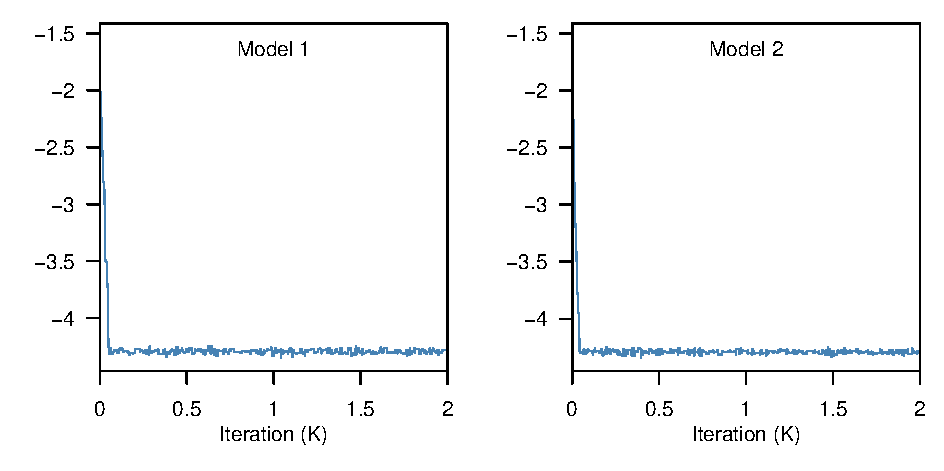
\includegraphics[width=\linewidth]{figures/03_NetworkModel/poc_traceplot_alpha.pdf}
    \caption{Trace plot of the baseline density parameter ($\alpha$) during the parameter recovery test. The chains, intentionally initialized at $\alpha=-2.0$, successfully demonstrate rapid convergence to the true parameter value ($\alpha \approx -4.29$) across both modeling frameworks.}
    \label{fig:poc_traceplot}
\end{figure}

\subsubsection{Adaptive MCMC Strategies}
To achieve practical computation times, simulations are conducted at a reduced scale of $N=1000$.
However, this reduction introduces a mathematical gap, or energy barrier, between the simulated statistics and the strict target distribution derived from the full dataset.
To overcome this barrier and ensure efficient parameter space exploration, we introduce an Adaptive MCMC framework.
This framework utilizes an Inflation factor to artificially widen the target covariance matrix during the initial stages.
Additionally, a Scaling factor is employed to dynamically adjust the proposal covariance matrix based on the empirical acceptance rate.

\paragraph{3.2.6.1 Model 1: Hybrid Two-Stage Scheduling}\mbox{}\\
The stochastic likelihood evaluation in Model 1 imposes a severe computational bottleneck if executed naively.
To optimize the trade-off between inference accuracy and computational cost, we designed a Two-Stage Adaptive MCMC architecture.
Phase 1 (Exploration) utilizes a computationally efficient single simulation ($n_{\text{sim}}=1$) alongside a gradually decreasing Inflation factor.
This phase rapidly explores the parameter space and learns an optimized proposal covariance matrix.
Phase 2 (Final Sampling) inherits this learned covariance matrix and executes the final sampling against the strict target (Inflation = 1).
By employing $n_{\text{sim}}=60$ simulations per step in this final phase, the stochastic noise is effectively smoothed without compromising the overall computational feasibility.

\begin{algorithm}[H]
\caption{Hybrid Two-Stage Adaptive MCMC for Model 1 (Stochastic Evaluation)}
\begin{algorithmic}[1]
\Require Initial parameters $\boldsymbol{\theta}_0$, Target statistics $\boldsymbol{\mu}_{\text{target}}, \boldsymbol{\Sigma}_{\text{target}}$
\Require Schedule of Inflation factors $\{I_1, I_2, \dots, I_S\}$ where $I_S = 1$
\Ensure Samples from the posterior distribution $p(\boldsymbol{\theta} \mid \text{Data})$

\Statex \textbf{Phase 1: Exploration with Adaptive Covariance ($n_{\text{sim}} = 1$)}
\State Initialize proposal covariance $\boldsymbol{\Sigma}_{\text{prop}}$
\For{stage $s = 1$ to $S-1$}
    \State Set current target covariance: $\boldsymbol{\Sigma}_{\text{stage}} = I_s \cdot \boldsymbol{\Sigma}_{\text{target}}$
    \For{iteration $i = 1$ to $M_{\text{stage}}$}
        \State Propose $\boldsymbol{\theta}^* \sim \mathcal{N}(\boldsymbol{\theta}_{i-1}, \boldsymbol{\Sigma}_{\text{prop}})$
        \State Generate a single network $\mathcal{G}^*$ given $\boldsymbol{\theta}^*$
        \State Compute summary statistics $S(\mathcal{G}^*)$
        \State Evaluate stochastic likelihood $\mathcal{L}(\boldsymbol{\theta}^*)$
        \State Accept/Reject $\boldsymbol{\theta}^*$ via Metropolis-Hastings ratio
    \EndFor
    \State Extract valid posterior samples $\boldsymbol{\Theta}_{\text{valid}}^{(s)}$ after burn-in
    \State Update $\boldsymbol{\Sigma}_{\text{prop}} \gets \mathrm{Cov}(\boldsymbol{\Theta}_{\text{valid}}^{(s)}) \cdot \text{ScalingFactor}$
\EndFor

\Statex \textbf{Phase 2: Final Sampling with LogSumExp Stabilization ($n_{\text{sim}} = 60$)}
\State Set target covariance strictly to $I_S = 1$: $\boldsymbol{\Sigma}_{\text{final}} = \boldsymbol{\Sigma}_{\text{target}}$
\For{iteration $i = 1$ to $M_{\text{final}}$}
    \State Propose $\boldsymbol{\theta}^* \sim \mathcal{N}(\boldsymbol{\theta}_{i-1}, \boldsymbol{\Sigma}_{\text{prop}})$
    \State Generate $n_{\text{sim}}=60$ independent networks $\mathcal{G}^*_1, \dots, \mathcal{G}^*_{60}$
    \State Compute log-likelihoods $LL_k$ for each $S(\mathcal{G}^*_k)$ against $\boldsymbol{\Sigma}_{\text{final}}$
    \State Approximate expected log-likelihood via LogSumExp: $\mathcal{L}_{\text{LSE}}(\boldsymbol{\theta}^*) = \max(LL) + \log \left( \frac{1}{60} \sum \exp(LL_k - \max(LL)) \right)$
    \State Accept/Reject $\boldsymbol{\theta}^*$ via Metropolis-Hastings ratio
\EndFor
\State \Return Final stationary chain from Phase 2
\end{algorithmic}
\end{algorithm}


\paragraph{3.2.6.2 Model 2: Unitary Adaptive Process}\mbox{}\\
As established in Section 3.2.5.2, the deterministic likelihood evaluation in Model 2 is free from simulation-induced noise.
Consequently, the chain stalling phenomenon observed in stochastic evaluation does not occur.
This renders the Two-Stage hybrid approach unnecessary for Model 2.
Instead, we employ a streamlined unitary adaptive process utilizing a standard covariance updating scheme.
This deterministic algorithm efficiently traverses the high-dimensional parameter space and achieves rapid convergence.

\begin{algorithm}[H]
\caption{Adaptive MCMC for Model 2 (Deterministic Evaluation)}
\begin{algorithmic}[1]
\Require Initial parameters $\boldsymbol{\theta}_0$, Target statistics $\boldsymbol{\mu}_{\text{target}}, \boldsymbol{\Sigma}_{\text{target}}$
\Require Pre-sampled CRN matrix $\mathbf{U}$ for latent variables $Z_i \sim \mathcal{N}(0,1)$
\Require Schedule of Inflation factors $\{I_1, I_2, \dots, I_S\}$ where $I_S = 1$
\Ensure Samples from the posterior distribution $p(\boldsymbol{\theta} \mid \text{Data})$

\State Initialize proposal covariance $\boldsymbol{\Sigma}_{\text{prop}}$
\For{stage $s = 1$ to $S$}
    \State Set current target covariance: $\boldsymbol{\Sigma}_{\text{stage}} = I_s \cdot \boldsymbol{\Sigma}_{\text{target}}$
    \For{iteration $i = 1$ to $M_{\text{stage}}$}
        \State Propose $\boldsymbol{\theta}^* \sim \mathcal{N}(\boldsymbol{\theta}_{i-1}, \boldsymbol{\Sigma}_{\text{prop}})$
        \State Analytically compute expected network statistics via LLN given $\mathbf{U}$ and $\boldsymbol{\theta}^*$
        \State Evaluate deterministic likelihood $\mathcal{L}(\boldsymbol{\theta}^*)$
        \State Accept/Reject $\boldsymbol{\theta}^*$ via Metropolis-Hastings ratio
    \EndFor
    \State Extract valid posterior samples $\boldsymbol{\Theta}_{\text{valid}}^{(s)}$ after burn-in
    \State Update $\boldsymbol{\Sigma}_{\text{prop}} \gets \mathrm{Cov}(\boldsymbol{\Theta}_{\text{valid}}^{(s)}) \cdot \text{ScalingFactor}$
\EndFor
\State \Return Final stationary chain from stage $S$
\end{algorithmic}
\end{algorithm}


\subsubsection{MCMC Diagnostics (Convergence Check)}
To validate the soundness of the proposed inference engine, the stationarity and convergence of the MCMC chains were rigorously assessed using both visual and quantitative diagnostics.
Visual inspection was conducted using trace plots to confirm optimal, caterpillar-like mixing across the parameter space.
Quantitatively, convergence across multiple independent chains was evaluated using the Gelman-Rubin potential scale reduction factor ($\hat{R}$).
A threshold of $\hat{R} < 1.1$ was established to mathematically ensure that all chains successfully converged to the same stationary posterior distribution.
Furthermore, the Effective Sample Size (ESS) was calculated for each parameter to verify that a sufficient number of independent samples were drawn, minimizing the impact of autocorrelation.
Across all final inference runs for Model 1, Model 2A, and Model 2B, every parameter successfully achieved $\hat{R} \le 1.02$.
Additionally, the ESS values substantially exceeded standard minimum thresholds, ranging from approximately 800 to over 2000, thereby guaranteeing highly robust and reliable posterior estimates.

\paragraph{3.2.7.1 Diagnostics for Model 1: Overcoming Stochasticity}\mbox{}\\
Figure \ref{fig:model1_comparison} illustrates the trace plot transition for the baseline density parameter ($\alpha$) during the Model 1's Phase 1 inference.
As intended by the hybrid architectural design, Phase 1 facilitated broad parameter exploration while suppressing computational costs.
However, at the final stage of Phase 1 (Stage 6, Inflation = 1), the chain exhibits severe stagnation, where the trace plot becomes rigidly flat.
This failure occurs because, with $n_{\text{sim}}=1$, the stochastic noise of the likelihood estimator is too large relative to the strict target distribution, leading to a near-zero acceptance rate.
Upon transitioning to Phase 2 ($n_{\text{sim}}=60$, Inflation = 1), this stochastic noise was successfully smoothed using the LogSumExp stabilization.
This stabilization allowed the chain to immediately escape stagnation and sample consistently from the target posterior distribution.
This empirical evidence clearly demonstrates the critical necessity of the Two-Stage approach for stochastic network models.

\begin{figure}[H]
    \centering
    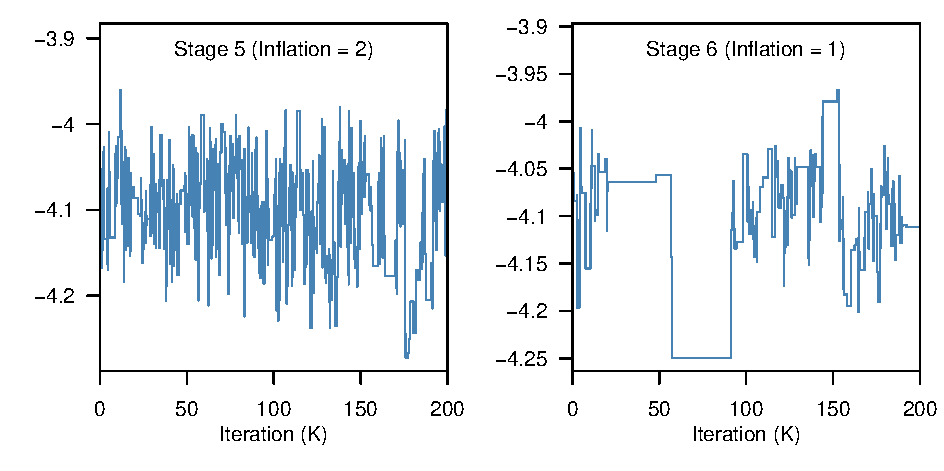
\includegraphics{figures/03_NetworkModel/model1_comparison_traceplot_alpha.pdf}
    \caption{Trace plot comparison for parameter $\alpha$ in Model 1, demonstrating the severe stagnation in Phase 1 (Stage 6: Inflation = 1, $n_{\text{sim}}=1$). The chain completely stalls due to stochastic noise exceeding the strict target tolerance.}
    \label{fig:model1_comparison}
\end{figure}

Figure \ref{fig:model1_stationary} presents the stationary trace plots for the four selected parameters ($\alpha$, $\phi_{ff}$, $\theta$, $\sigma_{re}$) throughout Phase 2.
The robust, caterpillar-like mixing observed across all four dimensions confirms that the $n_{\text{sim}}=60$ configuration provides sufficient likelihood stabilization.
Consequently, the MCMC algorithm successfully yielded a precise and fully converged posterior distribution for the stochastic baseline model.

\begin{figure}[H]
    \centering
    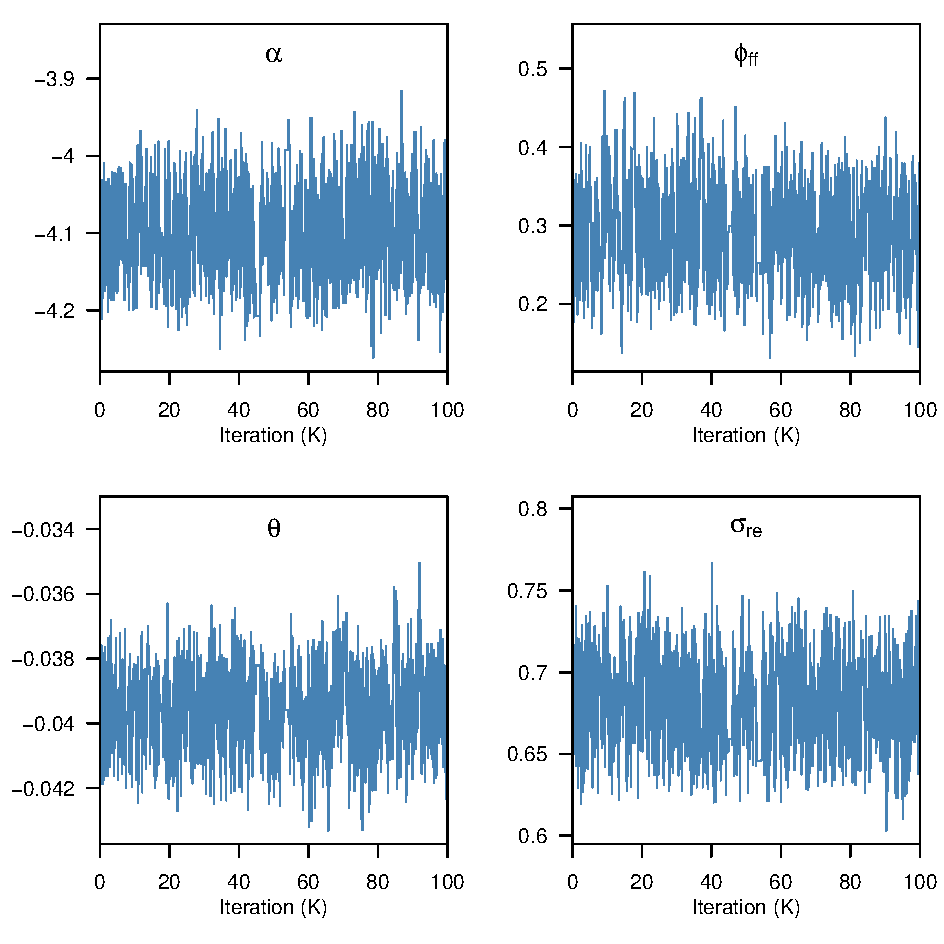
\includegraphics{figures/03_NetworkModel/model1_singlestage_traceplot.pdf}
    \caption{Stationary trace plots for the four primary parameters ($\alpha, \phi_{ff}, \theta, \sigma_{re}$) in Model 1 during Phase 2 ($n_{\text{sim}}=60$).
The consistent mixing across all dimensions indicates successful convergence to the posterior distribution.}
    \label{fig:model1_stationary}
\end{figure}


\paragraph{3.2.7.2 Diagnostics for Model 2: Deterministic Convergence}\mbox{}\\
For Model 2, the MCMC diagnostics confirm highly efficient and stable convergence due to the deterministic evaluation scheme.
Figure \ref{fig:model2_diagnostics} presents the trace plots for representative parameters of Model 2B.
These parameters capture key structural dimensions, including baseline density ($\alpha$), structural hierarchy ($\gamma_{\text{pri\_low}}$), attribute homophily ($\phi_{\text{mm}}$), and household generational heterogeneity ($\sigma_{\text{hhd}}$).
Unencumbered by probabilistic simulation noise, the parameter chains exhibit rapid mixing and establish a stationary distribution seamlessly within a single adaptive stage.
Comprehensive trace plots for all parameters across the variations are provided in the Appendix.

\begin{figure}[H]
    \centering
    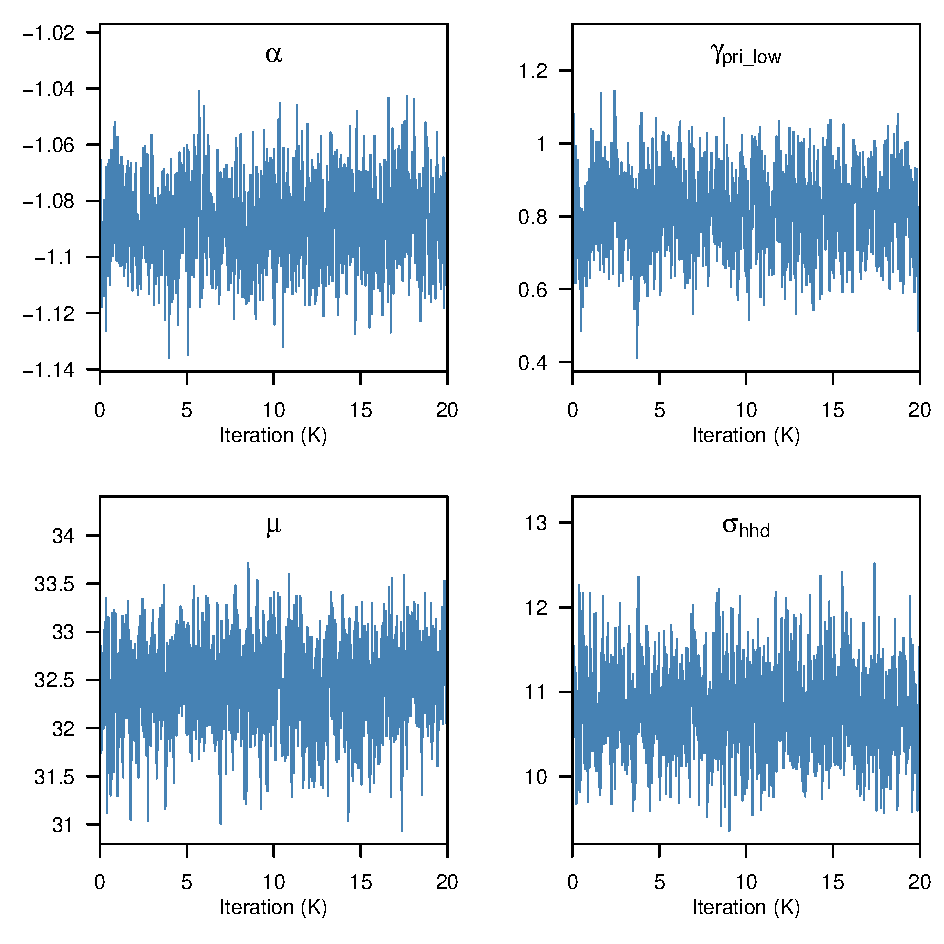
\includegraphics{figures/03_NetworkModel/model2b_singlestage_traceplot.pdf}
    \caption{MCMC diagnostic trace plots for representative parameters ($\alpha$, $\gamma_{\text{pri\_low}}$, $\phi_{\text{mm}}$, $\sigma_{\text{hhd}}$) in Model 2B, showing rapid and stable convergence.}
    \label{fig:model2_diagnostics}
\end{figure}